\documentclass{article}
\usepackage[utf8]{inputenc}
\usepackage{fixltx2e}
\usepackage{amsmath}
\usepackage{array}
\usepackage{graphicx}
\usepackage{algorithm}
\usepackage{algorithmic}

\DeclareMathOperator*{\argmax}{argmax}
\graphicspath{ {./} }

\title{Spam Filter with Naive Bayes}
\author{xu000159 }
\date{December 2020}

\begin{document}

\maketitle

\begin{abstract}
   Despite being one of the most technologically advanced nations, the US still suffers a disproportionately large amount of lost work hours due to spam. One of the simplest ways to curb this problem is through a Naive Bayesian spam filter. In this paper, the ideas behind Naive Bayes and different Bayesian classification methods will be explored, including multinomial, Gaussian, and Bernoulli classifiers. In addition, several different augmentations that can be integrated into the base algorithm will be analyzed. These augmentations include n-grams, word stemming, stop-words, and TF-IDF. Different classifier/augmentation combinations were tested on a Kaggle spam-ham email data set, with performance being measured based on number of undetected spam and false positives. Finally, these performance numbers will be discussed, and possible other additions will be explored.
\end{abstract}

\section{Introduction}
\begin{paragraph}
With email still being the primary method of communication in the corporate world, the relative purity of our email network is of vital importance. The security and dependability of a communication framework is vital to business, especially when many interactions within and between businesses are done via email communication. Unfortunately, things like spam and malicious emails can drown out important emails, as well as cause damage via virus and other malicious software. 
\end{paragraph}
\begin{paragraph}
With this issue affecting something as core as the email network of business-people, spam mail is bound to cause disruption to the operation of business. According to DataProt, spam email costed businesses an estimated 20.5 billion dollars in 2012. 
\cite{budanovic_letic_jovanovic_2020}
These costs include the time wasted wading through these spam emails as well as the cost of deletion and prevention. Furthermore, these spam mails can be sent by spam bots by the thousands at no cost to spammers. This creates a big issue for normal users: spammers and advertisers are able to endlessly send spam mail at no cost, rendering even one mail opened a success. Meanwhile, users who don't wish for these mails have to take on the burden of deleting and blocking future spam mail. It is only natural to then recognize the value of a spam filter, helping average users tidy up their inbox as well as potentially averting damage for companies.
\end{paragraph}
\begin{paragraph}
Fortunately, there are many options for filtering spam. One common way is to filter by sender. This usually comes in the form of filtering lists, where email is automatically rejected or blocked if its sender is from a known list of spammers. These lists can be of a variety of different types: whitelists, blacklists, community-maintained lists, etc. Sender-based methods usually require user reports of consistent "spammer" senders, as it is hard to draw conclusions based on senders themselves.
\end{paragraph}
\begin{paragraph}
The types of filters that will be explored in this paper fall under the category of content-based filtering, where an email is kept or discarded based on it's textual contents. Unlike sender-based filtering, content-based filtering will allow the spam to reach your inbox before taking action. Unlike sender-based filtering, content-based filtering can take a more mathematical approach to determining spam, since spam emails are directly defined by its content. Most content-based approaches will try to vectorize the email's contents into numbers, whether through heuristics, tokenization, etc. With the email represented as some collection of numbers, the use of algorithms can be introduced to analyze and conclude whether an email is spam or not.
\end{paragraph}
\begin{paragraph}
The content-based approach that this paper will examine is the Bayesian Filter. The Bayesian filter uses mathematical probability with previously seen email data to determine whether new emails are spam or not. At its core, Bayesian Filter follows Bayes' Theorem, that is:
\begin{equation}
 P(class|data)=\frac{P(data|class)P(class)}{P(data)}
\end{equation}
Which, at a high level, predicts the probability and email being spam based on the frequencies and probabilities of spam words with the general probability of spam.
\end{paragraph}
\begin{paragraph}
Other ways of eliminating spam without the use of a filter exist. These methods usually transfer the recipient's burden of receiving the email to the sender. This usually means that the sender or ISP must instead handle some sort of computation in order to send the email. This could mean that senders must provide authentication, paying fees to ISP to whitelist send requests in the thousands, etc. This paper will only focus on the mathematical techniques used in filtering, as these spam methods focus on an entirely different social matter.
\end{paragraph}

\section{Related Work}
\begin{paragraph}
When talking about automated program effectiveness, it is useful to establish a baseline to compare machine performance to. For spam filtering, this would be the manual labor of hand-filtering spam. While it's obvious that hand-filtering spam is a last resort, it is useful to recognize it's pros and cons to better create a solution. For manual filtering, the risks are pretty low, but so is the reward. Most people are able to determine spam and malicious emails at a very high accuracy, so very few mistakes are made. On the other hand, manual filtering is very costly in time and effort wasted in the workplace. Therefore, machine filters should be able to make improvements primarily in time, without sacrificing the already-high human accuracy.
\cite{cormack_2008}
\end{paragraph}
\begin{paragraph}
The first class of content-based filters that will be examined is of the "human supervised" variety. These filters operate mainly based on human knowledge of common spam traits, rather than a machine being able to learn these traits on its own. A basic form of this kind of filter is a word-based filter. This kind of filter looks to block emails based on common spam words, such as "free" or "discount". Although this filter is very simple to implement, it has the obvious downside of creating a lot of false positives. Business emails could easily contain common words found in spam, but it was the content of the email as a whole that distinguished it as "not spam". Simple models like word-based filtering does not account for content as a whole. The next level in content-based filtering would be a heuristic filter. A heuristic filter rates high indicating spam words such as "Nigerian prince" with a high score, and rates more common email words like "Regards" with low scores. The filter then adds up the total score of the email and determines if it's above some "spam" threshold. This takes a more holistic view on the email, but is still able to be sidestepped by spammers by avoid common "spam" words. 
\cite{gomez2000combining}
\end{paragraph}
\begin{paragraph}
Some sender-based filters of this class include blacklists, whitelists, and a special real-time blackhole list. All of these methods seek to filter spam in the same way: by recognizing frequent spam-sending addresses and blocking those addresses. Blacklists block everything on the list, whitelists only allow mail from the list, and real-time blackhole uses a blacklist maintained by a third party. These type of filters fall under a wide umbrella that is filtering by sender. 
\end{paragraph}
\begin{paragraph}
The other class of automatic filtering is that which includes machine learning. In the human supervised filtering, programs were given the common spam words and phrases and were in charge of determining spam based on the frequencies of these phrases. In machine learning filtering, the program will be able to determine these keywords on its own through supervised learning on available spam datasets.
\end{paragraph}
\begin{paragraph}
One popular machine learning technique is feature engineering. This type of filtering is especially effective in SNS spam, where each message is accompanied by a plethora of sender data. For problems that involve very rich data, feature engineering looks to extract the most important parts to use machine learning with. For SNS data, this means extracting information from the message (punctuation, uppercase, etc.) recipient (sex, age, country, friends on the app, etc), and sender (username, IP, account lifetime, etc.). These features can then be vectorized and used in a machine learning model. 
\cite{lupher1feature}
\end{paragraph}
\begin{paragraph}
Another universal learning technique is using k-nearest neighbors. Simply, this method attempts to find the k most related messages to any input message, and if the ratio of spam to normal emails is above some threshold, the input message is then classified as spam. Furthermore, there are many different ways to calculate "relatedness". Some methods include Euclidean distance, or the linear distance in Euclidean space, and cosine similarity, which will find the angular distance between two feature vectors. In a study by Tretyakov, emails were converted into feature vectors on word frequencies, and then used hyperplane distance to separate spam from normal emails. 
\cite{budanovic_letic_jovanovic_2020}
\end{paragraph}
\begin{paragraph}
This paper will focus on more statistical machine learning models. Specifically, we will be focusing on the Naive Bayes method. As explained earlier, Naive Bayes seeks to statistically determine the probability of a certain email being spam using Bayes Rule. The term of interest from the previously mentioned formula is the
\begin{equation}
    P(data|class) = P(data|f_1, f_2, ..., f_d) = \prod_{i=1}^{d} P(data|f_i)
\end{equation}
or the probability of given data coming from a certain class. There are multiple different assumptions that can be made about the distribution of this term, and those different assumptions will constitute entirely different statistical models. For example, there is a multinomial, Gaussian, and Bernoulli Naive Bayes, each assuming its corresponding distribution for features. For this experiment, a Multinomial Naive Bayes model will be used.
\cite{kibriya2004multinomial}
\cite{metsis2006spam}
\end{paragraph}

\section{Approach}
\begin{paragraph}
Starting with the spam email dataset, the first goal is to transform the textual data into some kind of feature vector. In this experiment, several different vectorization techniques are tested. The base algorithm used is simple tokenization. Tokenization involves splitting the text email into single words, and then storing the counts of each word as features. For example, the phrase "red red blue green green" would tokenize into [2 1 2], representing the frequencies for red, blue, and green, respectively. This is the "bag of words" model. However, there is a lot of room for improvement. Firstly, because every unique word in every email in the dataset is stored, there should be some sort of selection of the k top features to have the model run in a decent time. For this experiment, that k is 3000. Second, common, meaningless words such as "a" and "is" are removed based on a stop words list. Next, a stemmer is used to normalize common morphological and inflections in words. For example, "go", "going", and "gone" would be considered different features without a stemmer, but they are conjugations of the same word "go". Next, n grams are used to preserve adjacent ordering of related words. For example, the words "public" and "health" have different meaning when next to each other in text, and the introduction of n grams will help preserve that order in vectorization. Finally, instead of simply computing counts, we can also compute the TF-IDF of a term, or it's relevancy in a document within a collection of documents. These are outlined in the CountVectorizer and TfidfVectorizer from scikit-learn, respectively.
\end{paragraph}
\begin{paragraph}
While stop word removal might be a minor improvement, stemming and n-grams will vastly improve the quality of the vectorized data. n-grams preserve some of the information in ordering, and help reduce the sparsity of the vectorized data. Furthermore, n-grams can also be used on the character level. This further reduces the sparsity of the data matrix due to the fact that there aren't as many character combinations as word combinations. Character-wise n-grams also have the benefit of ignoring grammatical errors, although such errors might be useful in other areas of determining spam.
\cite{10.1007/11752912_12}
\end{paragraph}

\begin{paragraph}
Next, we will use the Multinomial Naive Bayes model to find the likelihood of an email being spam. Combining previously mentioned equations, we have the probability of spam being
\begin{equation}
    P(class|data)=\frac{P(data|class)P(class)}{P(data)} = \frac{\prod_{i=1}^{d} P(data|f_i)P(class)}{P(data)}
\end{equation}
where f\textsubscript{i} is the ith word in the vectorized feature vector. Given that we have two classes "spam" and "not spam", the predicted class of a given email would be
\begin{equation}
    Y_{pred} = \argmax_{class} P(class|data)
\end{equation}
after simplifying, Y\textsubscript{pred} becomes
\begin{equation}
    \argmax_{class} \frac{\prod_{i=1}^{d}P(data|f_i)P(class)}{P(data)}
\end{equation}
because we are interested in the maximum class probability, we can eliminate the P(data) denominator, giving
\begin{equation}
    \argmax_{class} \prod_{i=1}^{d}P(data|f_i)P(class)
\end{equation}
taking the log of the geometric sum then gives
\begin{equation}
    \argmax_{class}  log(\sum_{i=1}^{d}P(data|f_i) + P(class))
\end{equation}
Then, using Multinomial probability density for P(data|f\textsubscript{i}) and the training class frequency for P(class), we can find out the maximum likelihood estimate for the predicted class. In this case, our only two classes are spam and not spam.
\end{paragraph}

\section{Experiment Design and Results}
\begin{paragraph}
To train the model, a Kaggle spam-ham csv dataset with 5731 examples was used. The Naive Bayes model I implemented was actually a wrapper for a scikit-learn MultinomialNB model. My wrapper class was in charge of converting the csv data into vectorized form based on the options specified in the constructor(stop words, stemming, etc.).
\end{paragraph}

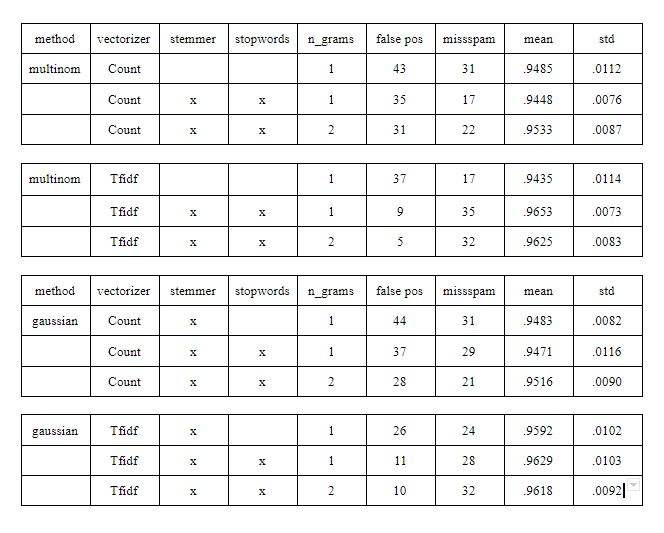
\includegraphics[scale=.63]{table1.JPG}
\begin{paragraph}
\usepackage{}{Table 1: Performance of different method combinations}
\end{paragraph}

\begin{paragraph}
When evaluating the NaiveBayes wrapper model, scikit-learn and its k-cross validation capabilities were used. First, the data was split into five equal portions with k=5. For each configuration of the NaiveBayes model, the model would train itself on the four portions not selected, then test itself based on the selected portion, once for each portion. This way, there would be five different accuracy scores that would be averaged and reported as the mean and std. Similarly, the false positive and missspam would be averaged out to the nearest whole number. This would be repeated for each configuration of the NaiveBayes model, of which 12 were tested. 


\begin{algorithm}[H]
\caption{Experiment}
\begin{algorithmic} 
\STATE $dataset \leftarrow 'emails.csv'$
\FORALL{$method, configuration$ in $configurations$}
    \STATE $X, y \leftarrow vectorize(dataset, method)$
    \STATE $kfold\char`_split \leftarrow train\char`_test\char`_split(dataset)$
    \STATE $total\char`_performance \leftarrow [ ]$
    \FORALL{$X\char`_train, y\char`_train, X\char`_test, y\char`_test$ in $fold\char`_split$}
        \STATE $method(configuration).fit(X\char`_train, y\char`_train)$
        \STATE $y\char`_pred \leftarrow method.predict(X\char`_test)$
        \STATE $accuracy \leftarrow cross\char`_val\char`_score(method, y\char`_pred, y\char`_test)$
        \STATE $total\char`_performance \leftarrow total\char`_performance + accuracy$
    \ENDFOR
    \STATE $average\char`_performance \leftarrow mean(total\char`_performance)$
    \STATE $print(average\char`_performance[false\char`_positives])$
    \STATE $print(average\char`_performance[missed\char`spam])$
    \STATE $print(average\char`_performance[mean])$
    \STATE $print(average\char`_performance[std])$
\ENDFOR
\end{algorithmic}
\end{algorithm}
\end{paragraph}

\begin{paragraph}
In total, the MutinomialNB, GaussianNB classifiers was tested with both the Count and TfidfVectorizer with various different configurations of stemming, using stopwords, and having n-grams=2. False positives indicated that the actual email was not spam, but the classifier incorrectly predicted that it was spam. This is the most severe type of error, because a wrongly marked spam email could be a very important business email that would be ignored. Missed spam indicates that the actual email is spam, but was marked as not spam. Relative to a false positive, this is just a minor inconvenience that a spam email shows up in an inbox on accident.
\end{paragraph}

\section{Analysis}
\begin{paragraph}
In general, accuracies improved with the addition of stemmers, stopwords, and n-grams of 2. Additionally, false positives decreased dramatically with the addition of extra configurations. The best performing method was the multinomial with the tfidf vectorizer and n-grams=2. Interestingly enough, the Gaussian method with the same configuration performed very similarly. This must indicate that the P(data|class) was modeled similarly between the two statistical distributions. At least the performance increased with the addition of extra configurations that were described before.
\end{paragraph}
\begin{paragraph}
However, missed spam tended to hover around 20 to 30 for all tests, and did not follow any pattern with regard to either the method nor the configurations. However, this may be due to the nature of the training dataset. Less than a third of the entries in the 'emails.csv' training set were actually spam, so perhaps the fitted classifier was hesitant to mark any spam. This is further confirmed by the low false positive rate, a maximum of 44 out of the 1046 y-test datapoints in the k-fold cross validation, a mere 2 percent false positive rate.
\end{paragraph}
\begin{paragraph}
What was also unexpected was the small discrepancy between the CountVectorizer and the TfidfVectorizer. Since the TfidfVectorizer takes into account the term frequency(count) and the relative importance of that term in the big picture of the whole dataset. However, this extra information only contributed to a maximum 2 percent increase in accuracy for the same method and configuration. Once again, this is most likely due to the nature of the dataset. If the TfidfVectorizer scales the CountVectorizer by the inverse document frequency, then that idf term must be fairly similar across all terms, indicating a potentially faulty dataset.
\end{paragraph}
\begin{paragraph}
Overall, these fairly similar results may have been due to the way in which the wrapper class was coded. The NaiveBayes wrapper that was used mainly delegated functionality into the underlying MultinomialNB or GaussianNB, or left functionality to scikit-learn's under-the-hood configurations. I wasn't able to figure out many of the intricacies of stop word and stemming configurations, so a lot of the work was left into the built in functions. This, along with only using a single email dataset, was most likely the reason for the underwhelming results.
\end{paragraph}
\begin{paragraph}
With regard to Graham's results, the advertised 0 percent false positive rate was almost achieved. The lowest false positive count was the multinomial tfidf method with full configurations, with a rate of 0.48 percent. Unfortunately, the false negative rate in this experiment was nowhere close to the advertised 0.5 percent. It is worth mentioning, however, that Graham trained and tested his algorithms fully within his own inbox. In fact, the method that he used may have overfitted his inbox emails that were most likely consistent in topic and content, based on his comment that many emails in his inbox are related to programming. In fact, this is the reason why Graham's results are drastically different: He trained and tested exclusively on his own dataset, which consisted of emails that did not differ much in content. On the other hand, while only one dataset was used in this experiment, the actual emails used were diverse in both spam content and regular email content. All in all, this experiment proved to be consistent with what is known about these filtering techniques, and more testing should be done on different datasets with slightly different implementations.
\cite{a_plan_for_spam}
\end{paragraph}

\section{Conclusion and Future Work}
\begin{paragraph}
In conclusion, the Tfidf, high n gram count, stemmer, and stop words improves spam detection performance by a decent amount, 2 percent in this experiment. Furthermore, for out dataset, the difference between the Multinomial model and the Gaussian model is fairly small. Nevertheless, the most effective configuration was the Multinomial Naive Bayes with stopwords, stemming, and n gram=2.
\end{paragraph}
\begin{paragraph}
In the future, it will definitely be beneficial to have specialized datasets that have separate trends within them. As demonstrated in Graham's results, general testing of the performance spam filtering will differ quite a bit when using a generalized, all-in-one dataset like this experiment versus the familiar, consistent inbox of Graham. In addition, more features should be tested in the future along with these specialized datasets to perhaps find which configurations are best for each type of inbox. For example, stemming may work better in a businessman's inbox because common phrases may be repeated, but Tfidf might show a drastically better performance in a social person's inbox due to the increased significance of the IDF term in relation to that person's diverse inbox.
\end{paragraph}
\begin{paragraph}
All in all, more testing should be done to produce significant results. There are plenty of different spam filtering techniques that were not explored in this experiment, such as linear classifiers, support vector machines, and much more.
\end{paragraph}


\bibliographystyle{abbrv}
\bibliography{./bibtex}
\end{document}
